%% =============================================================================
%%  Articulo en formato IEEE (clase IEEEtran, modo "journal")
%%  Compilar en Overleaf con pdfLaTeX. Documento principal: main.tex
%%  Bibliografia: referencias.bib (BibTeX, estilo IEEEtran)
%%  Las cifras del texto y las tablas de resultados las genera codigo/gen_tablas_opt.py
%%  (numeros.tex, tabla_*.tex) a partir de resultados/opt/evaluacion_final.json.
%% =============================================================================
\documentclass[journal]{IEEEtran}

% ---- Codificacion e idioma ---------------------------------------------------
\usepackage[utf8]{inputenc}
\usepackage[T1]{fontenc}
\usepackage[spanish,es-tabla,es-nodecimaldot]{babel}
\addto\captionsspanish{\renewcommand{\figurename}{Fig.}\renewcommand{\abstractname}{Abstract}}

% ---- Paquetes ----------------------------------------------------------------
\usepackage{cite}
\usepackage{amsmath,amssymb}
\usepackage{graphicx}
\usepackage{booktabs}
\usepackage[table]{xcolor}
\usepackage{array}
\usepackage{url}

\graphicspath{{figures/}}
% Generado por gen_tablas_opt.py (no editar a mano)
\newcommand{\DelayOfFijo}{13.81}
\newcommand{\DelayOfAct}{10.89}
\newcommand{\DelayOfActAf}{9.96}
\newcommand{\DelayOfMax}{31.20}
\newcommand{\DelayOfPap}{10.95}
\newcommand{\DelayOfPapAf}{9.69}
\newcommand{\DelayOfMdp}{9.35}
\newcommand{\DelayOfFlc}{9.14}
\newcommand{\DelayOfFlcC}{10.53}
\newcommand{\DelayOfMlp}{8.68}
\newcommand{\DelayOfMlpC}{10.17}
\newcommand{\DelayNvFijo}{12.31}
\newcommand{\DelayNvAct}{10.19}
\newcommand{\DelayNvActAf}{9.20}
\newcommand{\DelayNvMax}{23.48}
\newcommand{\DelayNvPap}{9.99}
\newcommand{\DelayNvPapAf}{9.05}
\newcommand{\DelayNvMdp}{8.47}
\newcommand{\DelayNvFlc}{8.33}
\newcommand{\DelayNvFlcC}{9.81}
\newcommand{\DelayNvMlp}{7.93}
\newcommand{\DelayNvMlpC}{9.56}
\newcommand{\DelayVaFijo}{12.29}
\newcommand{\DelayVaAct}{9.23}
\newcommand{\DelayVaActAf}{8.39}
\newcommand{\DelayVaMax}{16.94}
\newcommand{\DelayVaPap}{8.65}
\newcommand{\DelayVaPapAf}{8.02}
\newcommand{\DelayVaMdp}{7.94}
\newcommand{\DelayVaFlc}{7.33}
\newcommand{\DelayVaFlcC}{9.05}
\newcommand{\DelayVaMlp}{6.89}
\newcommand{\DelayVaMlpC}{8.81}
\newcommand{\DelaySaFijo}{40.67}
\newcommand{\DelaySaAct}{54.06}
\newcommand{\DelaySaActAf}{23.16}
\newcommand{\DelaySaMax}{350.99}
\newcommand{\DelaySaPap}{105.87}
\newcommand{\DelaySaPapAf}{62.14}
\newcommand{\DelaySaMdp}{23.11}
\newcommand{\DelaySaFlc}{48.73}
\newcommand{\DelaySaFlcC}{49.62}
\newcommand{\DelaySaMlp}{54.30}
\newcommand{\DelaySaMlpC}{232.71}
\newcommand{\RedFijo}{-26.1}
\newcommand{\RedAct}{0.6}
\newcommand{\RedActAf}{9.1}
\newcommand{\RedMax}{-184.9}
\newcommand{\RedPapAf}{11.5}
\newcommand{\RedMdp}{14.7}
\newcommand{\RedFlc}{16.6}
\newcommand{\RedFlcC}{3.8}
\newcommand{\RedMlp}{20.8}
\newcommand{\RedMlpC}{7.2}
\newcommand{\RedPapOf}{16.6}
\newcommand{\RedActAfOf}{8.3}
\newcommand{\RedPapNv}{16.6}
\newcommand{\RedActAfNv}{9.4}
\newcommand{\RedPapVa}{15.3}
\newcommand{\RedActAfVa}{12.7}
\newcommand{\RedPapSa}{54.0}
\newcommand{\RedActAfSa}{-110.4}
\newcommand{\ParMediaPap}{13.7}
\newcommand{\ParMejorPap}{16}
\newcommand{\ParPeorPap}{0}
\newcommand{\ParMinPap}{4.7}
\newcommand{\ParMaxPap}{28.2}
\newcommand{\ParMediaActAf}{10.8}
\newcommand{\ParMejorActAf}{12}
\newcommand{\ParPeorActAf}{2}
\newcommand{\ParMinActAf}{-2.1}
\newcommand{\ParMaxActAf}{23.6}
\newcommand{\ParMediaAct}{18.5}
\newcommand{\ParMejorAct}{16}
\newcommand{\ParPeorAct}{0}
\newcommand{\ParMinAct}{7.0}
\newcommand{\ParMaxAct}{31.8}
\newcommand{\ParMediaFijo}{32.8}
\newcommand{\ParMejorFijo}{16}
\newcommand{\ParPeorFijo}{0}
\newcommand{\ParMinFijo}{24.3}
\newcommand{\ParMaxFijo}{38.7}
\newcommand{\PdMaxDif}{0.7}
                          % cifras generadas desde los resultados

\newcommand{\fuente}[1]{\par\vspace{3pt}\noindent{\scriptsize\textit{Fuente:} #1\par}}
\renewcommand{\thetable}{\arabic{table}}
\newcommand{\qbar}{\bar{q}}              % tasa media de llegada (veh/s)
\newcommand{\FLC}{FLC-O}

% =============================================================================
\begin{document}

\title{Optimización de un controlador de semáforos de lógica difusa para una intersección aislada: más allá de la réplica del controlador de Pappis y Mamdani (1977)}

\author{Raul Nolberto Quispe Saya and Kevin Luis Valero Ccacya%
\thanks{R. N. Quispe Saya y K. L. Valero Ccacya pertenecen a la Escuela Profesional de Ingeniería Electrónica, Universidad Nacional de San Agustín de Arequipa, Arequipa, Perú (correos electrónicos: rquispesa@unsa.edu.pe, kvaleroc@unsa.edu.pe).}}

\markboth{Quispe Saya y Valero Ccacya: Optimización de un controlador difuso de semáforos}%
{Quispe Saya y Valero Ccacya: Optimización de un controlador difuso de semáforos}

\maketitle

% =============================================================================
\begin{abstract}
This paper starts from the replication of the 1977 Pappis--Mamdani fuzzy-logic traffic-signal controller for an isolated two-phase intersection and turns it into an optimization study. First, the delay measure is corrected to count all waiting time until the horizon. Second, a vectorized simulator is built that reproduces the reference simulator exactly (zero difference in six controllers) and runs about twenty times faster. Third, the optimal policy for known flows without look-ahead is computed by dynamic programming and used as a benchmark. Fourth, a 27-rule fuzzy controller (FLC-O) with singleton consequents is trained with CMA-ES; its membership functions, rules and look-ahead weights (42 parameters) are learned on random flows that are not those used for evaluation. On the 16 flow pairs of the original Table VIII, with 20 replications of 7200 s, FLC-O reduces the mean delay from \DelayOfPap{} to \DelayOfFlc{} s/veh (\RedFlc\,\%) with respect to the replicated controller, is significantly better in \ParMejorPap{} of 16 pairs and never significantly worse, and also improves a tuned actuated controller by \RedActAfOf\,\%. The gain holds on unseen flows and with time-varying demand. It relies on the 10-s look-ahead of arrivals that the original model already assumes: without it, the best learned controller improves the tuned actuated one by only \RedActMlpC\,\% (against \RedActAfOf\,\% for FLC-O with it). Near saturation the controllers are evaluated separately and the result is reported as a limitation.
\end{abstract}

\begin{IEEEkeywords}
Fuzzy logic control, Mamdani inference, CMA-ES, dynamic programming, traffic signal control, vehicle delay.
\end{IEEEkeywords}

\IEEEpeerreviewmaketitle

\noindent{\footnotesize\textbf{\textit{Resumen}---}Este artículo parte de la réplica del controlador de semáforos con lógica difusa de Pappis y Mamdani (1977) para una intersección aislada de dos fases y la convierte en un estudio de optimización. Primero se corrige la medida del retardo para que cuente toda la espera hasta el horizonte. Segundo, se construye un simulador vectorizado que reproduce exactamente al simulador de referencia (diferencia nula en seis controladores) y es unas veinte veces más rápido. Tercero, se calcula por programación dinámica la política óptima para caudales conocidos y sin vista adelante, que se usa como cota. Cuarto, se entrena con CMA-ES un controlador difuso de 27 reglas con consecuentes numéricos (FLC-O) cuyas funciones de pertenencia, reglas y pesos de la vista adelante (42 parámetros) se aprenden con caudales sorteados que no son los de la evaluación. En los 16 pares de caudales de la Tabla~VIII del original, con 20 réplicas de 7200\,s, FLC-O reduce el retardo medio de \DelayOfPap{} a \DelayOfFlc{}\,s/veh (\RedFlc\,\%) respecto del controlador replicado, es significativamente mejor en \ParMejorPap{} de 16 pares y nunca significativamente peor, y también mejora en \RedActAfOf\,\% a un actuado afinado. La ganancia se mantiene con caudales no vistos y con demanda variable. Depende de la vista adelante de 10\,s que el modelo original ya supone: sin ella, el mejor controlador aprendido mejora al actuado afinado solo en \RedActMlpC\,\% (frente a \RedActAfOf\,\% de FLC-O con ella). Cerca de la saturación los controladores se evalúan aparte y el resultado se presenta como limitación.\par}
\vspace{2pt}
\noindent{\footnotesize\textbf{\textit{Palabras clave}---}Control con lógica difusa, inferencia de Mamdani, CMA-ES, programación dinámica, control de semáforos, retardo vehicular.\par}

% =============================================================================
\section{Introducción}
\label{sec:intro}

\IEEEPARstart{E}{l} control de las señales luminosas de una intersección es uno de los problemas más estudiados de la ingeniería de tránsito. En la intersección aislada consiste en repartir el tiempo de verde entre las fases para reducir una medida de desempeño; la más habitual es el retardo medio por vehículo \cite{Pappis1977,Papageorgiou2003}. Los métodos clásicos fijan el ciclo y los verdes con los caudales medios \cite{Webster1958,Webster1966,Miller1963,Allsop1971}, los controladores actuados y adaptativos los modifican con detectores \cite{Hunt1982,Lowrie1982,Mirchandani2001}, y una tercera familia traduce el criterio de un operador a reglas lingüísticas ejecutadas con lógica difusa \cite{Zadeh1965,Zadeh1973,MamdaniAssilian1975}. Su referencia fundacional en tráfico es Pappis y Mamdani \cite{Pappis1977}: dos calles unidireccionales sin giros, un controlador que interviene a los 7, 17, 27, 37 y 47\,s del verde efectivo y decide con 25 reglas cuántos segundos extenderlo (de 1 a 10\,s) o si cambia de fase.

Un trabajo previo de los autores replicó ese controlador a partir de la publicación original, con una única fuente, y lo validó elemento por elemento (conjuntos, operadores, reglas y ejemplo trabajado) y con 20 réplicas estadísticas. La réplica dejó tres hechos. Primero, el controlador mejora al ciclo fijo de Webster en 16 de 16 combinaciones de caudal, como publicó el original. Segundo, frente a un actuado por detector, que el original no incluye, no es mejor en promedio. Tercero, sus reglas se afinaron por prueba y error en 1977, de modo que no hay razón para pensar que sean las mejores. Este trabajo pregunta cuánto puede mejorarse ese controlador si se optimizan sus parámetros y su estructura con un procedimiento reproducible, y contra qué referencias justas hay que medirlo.

Las contribuciones son:
\begin{enumerate}
\item Una medida del retardo que cuenta toda la espera hasta el horizonte y un simulador vectorizado que da, escenario por escenario, exactamente los mismos retardos que el de referencia y es unas veinte veces más rápido, lo que hace posible optimizar.
\item Una cota de lo alcanzable sin ver el futuro: la política óptima por programación dinámica para caudales conocidos, validada contra la simulación.
\item \FLC{}: un controlador difuso de 27 reglas, con consecuentes numéricos, que decide cada segundo y cuyos 42 parámetros se entrenan con CMA-ES; las reglas siguen siendo legibles.
\item Un protocolo sin fuga de información: entrenamiento con caudales sorteados, y prueba en los 16 pares de la Tabla~VIII del original y en conjuntos adicionales (caudales no vistos, demanda variable, cerca de la saturación), con estadística pareada.
\item Un análisis de qué información y qué diseño producen la mejora: vista adelante frente a causal, verde mínimo, número de reglas y comparación con una política neuronal.
\end{enumerate}

La Sección~\ref{sec:sota} revisa el estado del arte; la \ref{sec:modelo}, el modelo y la medida del retardo; la \ref{sec:pappis}, el controlador de Pappis y Mamdani; la \ref{sec:simulador}, el simulador vectorizado y la cota óptima; la \ref{sec:opt}, los controladores optimizados; la \ref{sec:protocolo}, el protocolo experimental; la \ref{sec:resultados}, los resultados; la \ref{sec:discusion} los discute y la \ref{sec:conclusiones} concluye.

% =============================================================================
\section{Estado del arte}
\label{sec:sota}

\subsection{Control de una intersección aislada}
El \emph{control de tiempo fijo} repite un plan calculado con los caudales medios; Webster \cite{Webster1958} dedujo el ciclo que minimiza el retardo, y Webster y Cobbe \cite{Webster1966}, Miller \cite{Miller1963}, Allsop \cite{Allsop1971} y TRANSYT \cite{Robertson1969} estudiaron sus ajustes. Su limitación es que los retardos reales exceden los óptimos cuando los caudales se apartan de los de diseño \cite{Pappis1977}. Un \emph{controlador actuado} prolonga el verde mientras los detectores ven llegadas, entre un mínimo y un máximo; los \emph{sistemas adaptativos} optimizan parámetros en línea: SCOOT \cite{Hunt1982}, SCATS \cite{Lowrie1982} y RHODES \cite{Mirchandani2001}; Papageorgiou \emph{et al.} \cite{Papageorgiou2003} revisan las estrategias urbanas. Un controlador de \emph{presión máxima} da paso al brazo con mayor presión y tiene garantías de estabilidad en redes \cite{Varaiya2013}. En todos ellos el desempeño estándar es el retardo medio por vehículo.

\subsection{Lógica difusa y control de semáforos}
Zadeh \cite{Zadeh1965,Zadeh1973,Zadeh1975} introdujo los conjuntos difusos, el enfoque lingüístico y la variable lingüística; Mamdani y Assilian \cite{MamdaniAssilian1975} los aplicaron al control de una planta, con el «y» como mínimo y el «si no» como máximo. Variantes posteriores son los consecuentes funcionales de Takagi y Sugeno \cite{TakagiSugeno1985} y la red adaptativa de Jang \cite{Jang1993}. En semáforos, Pappis y Mamdani \cite{Pappis1977} afinaron las reglas por prueba y error. Después, Trabia \emph{et al.} \cite{Trabia1999} proponen un controlador de dos etapas con detectores de lazo; Niittymäki y Pursula \cite{Niittymaki2000} desarrollan principios y algoritmos y citan una comparación de 1996 entre el algoritmo de Pappis y Mamdani y el principio de extensión \cite{Pursula1996}; Bingham \cite{Bingham2001} ajusta las funciones de pertenencia con una red neuronal y aprendizaje por refuerzo; y Murat y Gedizlioglu \cite{Murat2005} presentan FLMuSiC. Entre 2021 y 2026 siguen Ali \emph{et al.} \cite{Ali2021} (difuso con la fórmula de Webster en SUMO), Jiang \emph{et al.} \cite{Jiang2021} (esquema de dos etapas), Vuong \emph{et al.} \cite{Vuong2021} (ANFIS) y Shaheen \emph{et al.} \cite{Shaheen2026} (variantes intuicionista y de tipo 2). Estas obras conservan la estructura lingüística de Pappis y Mamdani pero ninguna optimiza, con un protocolo de prueba separado, el controlador original frente a un actuado afinado y una cota óptima.

\subsection{Aprendizaje por refuerzo y optimización de políticas}
Una línea paralela formula el control como decisión secuencial: Abdulhai \emph{et al.} \cite{Abdulhai2003} aplican \emph{Q-learning} a una intersección aislada y el aprendizaje profundo \cite{Mnih2015,Genders2016,Wei2018,Chu2020} se evalúa en simuladores y con datos reales; Noaeen \emph{et al.} \cite{Noaeen2022} y Michailidis \emph{et al.} \cite{Michailidis2025} lo revisan, y Vlasceanu \emph{et al.} \cite{Vlasceanu2025} contrastan un difuso con \emph{Q-learning}. Estos métodos aprenden la política de los datos pero dependen de la definición de estado y recompensa y de hiperparámetros cuya documentación incompleta dificulta comparar \cite{Henderson2018}. Aquí se usa una estrategia evolutiva, CMA-ES \cite{Hansen2001,Hansen2016}, para entrenar los parámetros de un controlador difuso y de una política neuronal: es una optimización de caja negra del retardo medio simulado, sin gradiente, adecuada para pocos parámetros y objetivos con escalones como el de decidir cuándo cortar el verde.

\subsection{Brecha}
Falta, en las fuentes consultadas, una comparación en la que el controlador difuso de 1977, su versión afinada y un difuso nuevo se midan con un mismo protocolo contra un actuado también afinado, una cota óptima y una política aprendida, separando entrenamiento, validación y prueba, y reportando cuánto de la mejora depende de ver el futuro cercano.

% =============================================================================
\section{Modelo de la intersección y medida del retardo}
\label{sec:modelo}

El modelo es el del original \cite{Pappis1977}: dos brazos unidireccionales sin giros que comparten un cruce, flujo de saturación $s=1$\,veh/s y un tiempo perdido de $5$\,s en cada cambio de fase (10\,s por ciclo). El tiempo avanza en pasos de 1\,s. En cada paso llega a lo sumo un vehículo al brazo $i$: $\alpha_n=1$ con probabilidad $\qbar_i$ (llegadas de Bernoulli). Durante el rojo nadie sale; durante el verde salen $s$ vehículos por segundo mientras haya cola, y un vehículo que llega con la cola vacía cruza sin esperar. Si $Q_{i,n}$ es la cola del brazo $i$ al final del segundo $n$, la espera total de todos los vehículos hasta el horizonte $H$ y el retardo medio por vehículo son
\begin{equation}
D=\sum_{n=0}^{H-1}\bigl(Q_{1,n}+Q_{2,n}\bigr),\qquad d_m=\frac{D}{\sum_{n<H}(\alpha_{1,n}+\alpha_{2,n})}.
\label{eq:dm}
\end{equation}
La primera igualdad es una deducción, no una convención: el retardo de un vehículo es el número de finales de segundo en que está en cola (de su llegada a su salida, o al horizonte si sigue en cola), y sumar primero por vehículo y luego por segundo, o al revés, da la suma de las colas, es decir, el área bajo las curvas de cola; la segunda es la definición de media. El original suma la espera de un vehículo cuando sale; los que siguen en cola al final del horizonte cuentan en el denominador y aportan cero, lo que subestima el retardo, en especial con colas largas. En este artículo el retardo es siempre \eqref{eq:dm}, que incluye la espera residual. Para el controlador de Pappis y Mamdani, la diferencia entre ambas convenciones es de \ResDifOf\,\% en promedio en el conjunto oficial (hasta \ResDifOfMax\,\% en un escenario) y de \ResDifSa\,\% en promedio cerca de la saturación (hasta \ResDifSaMax\,\%).

\begin{table}[t]
\centering
\caption{Notación (cada símbolo con un único significado)}
\label{tab:notacion}
\scriptsize
\setlength{\tabcolsep}{2.5pt}
\begin{tabular}{@{}cp{0.34\columnwidth}cp{0.34\columnwidth}@{}}
\toprule
Símbolo & Significado & Símbolo & Significado \\
\midrule
$\alpha_{i,n}$ & llegada al brazo $i$ en el segundo $n$ (0 o 1) & $\qbar_i$ & tasa de llegada (veh/s) \\
$Q_{i,n}$ & cola del brazo $i$ al final del segundo $n$ & $d_m$, $D$ & retardo medio (s/veh) y total (veh$\cdot$s) \\
$H$, $n_e$ & horizonte (s) y número de escenarios & $s$, $L$ & flujo de saturación y tiempo perdido por ciclo \\
$y_i$, $Y$, $C_0$, $g_i$ & razón de flujo, su suma, ciclo y verde de Webster & $T,E,A,Q$ & variables de Pappis y Mamdani (tiempo, extensión, arribos, cola) \\
$\gamma(e)$, $e^*$ & grado y extensión elegida ($0$: cambiar) & $Q_g$, $Q_r$ & colas del brazo con verde y del brazo en rojo \\
$G$, $R$, $V$ & demanda en verde, presión en rojo, verde transcurrido (\FLC{}) & $W_g(l)$, $W_r(l)$ & llegadas previstas en los $l$ s siguientes \\
$c_{ijk}$, $w_{ijk}$, $u$ & consecuente, fuerza de la regla y salida de \FLC{} & $\omega_k,\rho_k$ & pesos de la vista adelante \\
$g_{\min}$, $g_{\max}$ & verde mínimo y máximo & $J(\theta)$ & objetivo de entrenamiento \\
\bottomrule
\end{tabular}
\fuente{elaboración propia; los símbolos de Pappis y Mamdani \cite{Pappis1977} se conservan, salvo la tasa de llegada, que se escribe $\qbar_i$ para reservar $q$ a las colas.}
\end{table}

La línea base clásica es el ciclo fijo de Webster, con $y_i=\qbar_i/s$, $Y=y_1+y_2$, $L=10$\,s:
\begin{equation}
C_0=\frac{1.5\,L+5}{1-Y},\qquad g_i=\frac{y_i}{Y}\,(C_0-L),
\label{eq:webster}
\end{equation}
tomados de Webster \cite{Webster1958} tal como los imprime el original (p.~709), con los verdes redondeados al segundo más próximo. El reparto $g_i\propto y_i$ se deduce de igualar los grados de saturación de las dos fases, $X_i=y_iC/g_i$, con $g_1+g_2=C-L$; las constantes $1.5$ y $5$ del ciclo son un ajuste empírico de Webster y no se deducen. El ciclo fijo necesita conocer los caudales; los controladores de las secciones siguientes no los conocen.

% =============================================================================
\section{El controlador de Pappis y Mamdani}
\label{sec:pappis}

\subsection{Estructura}
\label{sec:estructura}
El controlador interviene a los 7, 17, 27, 37 y 47\,s del verde y decide la extensión $e^*\in\{0,1,\dots,10\}$ s del verde; $e^*=0$ cambia de fase y el verde máximo es de 57\,s. Usa cuatro variables sobre universos discretos: el tiempo $T$ y la extensión $E$ ($1$ a $10$\,s), los arribos $A$ ($1$ a $10$ veh en el brazo con paso) y la cola $Q$ ($4$ a $32$ veh en el brazo en rojo). Las reglas usan versiones monótonas de los conjuntos con dos operadores: si $x_0$ es el punto donde $\mu_A$ es máxima,
\begin{align}
\mu_{lt(A)}(x)&=\begin{cases}1-\mu_A(x), & x<x_0\\ 0, & x\ge x_0\end{cases} &
\mu_{mt(A)}(x)&=\begin{cases}0, & x<x_0\\ 1-\mu_A(x), & x\ge x_0\end{cases}
\label{eq:mtlt}
\end{align}
de modo que $lt(A)\cup mt(A)=\overline{A}$ y $lt(A)\cap mt(A)=\emptyset$ en todo el universo, incluido $x_0$, porque en cada $x$ solo una de las dos es no nula; \eqref{eq:mtlt} son las definiciones del original (p.~710). Las 25 reglas son «si $T=t$ y $A=mt(a)$ y $Q=lt(q)$ entonces $E=e$», con $E=T$, cinco por intervención. La contribución de la regla $j$ a la extensión $e$ es $\min\{\mu_{T_j}(e),\mu_{mt(A_j)}(a_e),\mu_{lt(Q_j)}(q_e),\mu_{E_j}(e)\}$, el grado es $\gamma(e)=\max_j$ de ellas, y la decisión es
\begin{equation}
e^*=\begin{cases}\max\{e:\gamma(e)=\gamma_{\max}\}, & \gamma_{\max}\ge 0.5\\ 0, & \gamma_{\max}<0.5\end{cases}
\label{eq:decision}
\end{equation}
La ecuación \eqref{eq:decision} reúne tres enunciados del original: se elige la extensión de mayor grado (p.~713), si todos son menores que 0.5 la fase cambia (p.~714) y, en un empate, se toma la mayor extensión (p.~714). La Fig.~\ref{fig:fuzzificacion} muestra los conjuntos con los valores impresos en el original.

\begin{figure*}[!t]
\centering
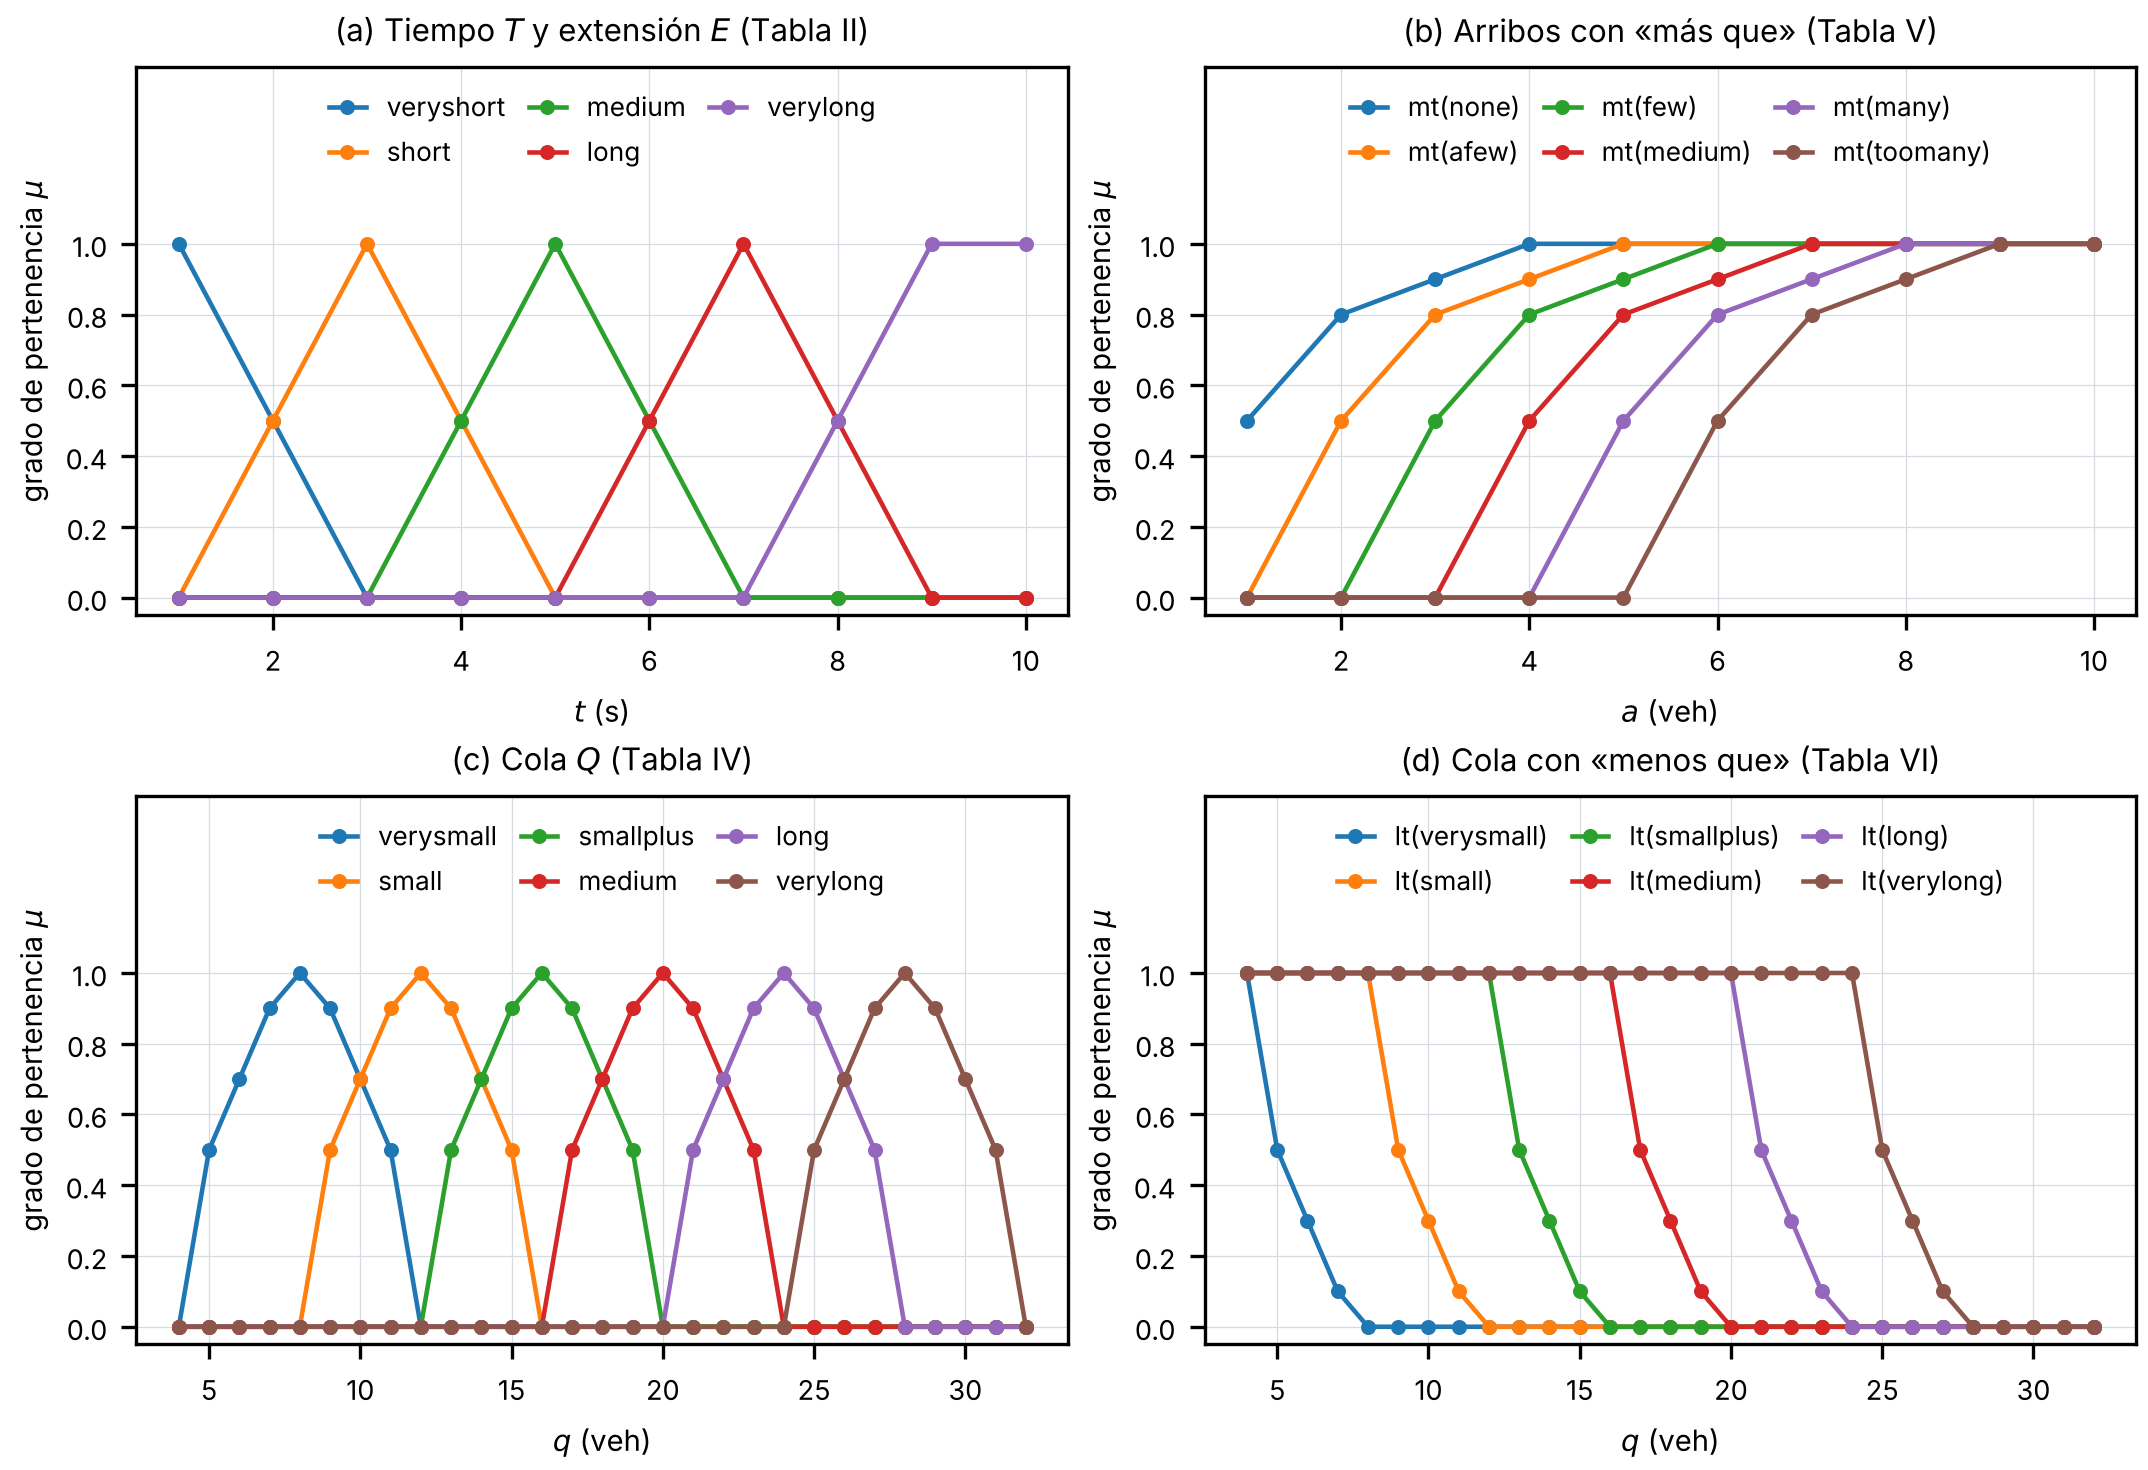
\includegraphics[width=\textwidth]{fig_fuzzificacion_ieee.png}
\caption{Curvas de fuzzificación del controlador de Pappis y Mamdani: (a) tiempo y extensión; (b) arribos con el operador «más que»; (c) colas; (d) colas con el operador «menos que». Trazadas con los valores impresos en el artículo original.}
\label{fig:fuzzificacion}
\end{figure*}

\subsection{Lectura de las entradas y réplica}
\label{sec:lecturas}
El original no dice cómo obtener $a_e$ y $q_e$ en una simulación. La réplica probó ocho lecturas y solo una, la \emph{calibrada}, reproduce sus resultados: $a_e=\min(e,\,Q_G+\sum_{i\le e}x_i)$, con $Q_G$ la cola del brazo con paso y $x_i$ las llegadas previstas en los $e$ segundos siguientes, y $q_e=Q_V$, los vehículos llegados al brazo en rojo desde que empezó el verde. Es una inferencia por falta de datos. Con ella, y con 20 réplicas de 7200\,s y números aleatorios comunes, la réplica reprodujo la tabla de validación del modelo con un error medio de 2.1\,\% y la mejora sobre el ciclo fijo en 16 de 16 combinaciones, con un error medio de 9.2\,\% frente a lo publicado. Todo lo que sigue usa esta lectura como controlador «Pappis y Mamdani».

Una propiedad del modelo importa para lo que sigue: las llegadas de los próximos 10\,s ($x_i$, $x'_i$) se suponen conocidas, como si detectores aguas arriba midieran los vehículos en tránsito. Es la \emph{vista adelante}. El controlador de la Sección~\ref{sec:opt} la conserva, y la Sección~\ref{sec:resultados} mide cuánto de su mejora depende de ella.

% =============================================================================
\section{Simulador vectorizado y cota óptima}
\label{sec:simulador}

\subsection{Simulador vectorizado}
\label{sec:vectorizado}
Optimizar exige evaluar un controlador en cientos de escenarios miles de veces. Se reescribió el simulador para simular $n_e$ escenarios a la vez con arreglos de NumPy: como \eqref{eq:dm} solo necesita las longitudes de cola, no se mantiene la lista de llegadas de cada vehículo, y las llegadas se generan con el mismo generador y las mismas semillas que el simulador de referencia. La equivalencia es exacta: en 8 escenarios de 2400\,s, con el ciclo fijo (dos redondeos), el actuado y el difuso de Pappis y Mamdani (dos lecturas), el retardo coincide con diferencia nula con las dos convenciones (\texttt{test\_sim\_batch.py}). Con un núcleo y 320 escenarios de 7200\,s, el difuso de Pappis y Mamdani tarda unos 3.3\,s (10\,ms por escenario) frente a unos 230\,ms por escenario con el simulador de referencia, unas veinte veces menos.

\subsection{Cota óptima por programación dinámica}
\label{sec:pd}
Para saber cuánto puede mejorarse sin ver el futuro se calcula la política óptima de un proceso de decisión de Markov \cite{Puterman1994} con un paso de 1\,s. El estado es $(Q_1,Q_2,\text{fase})$ en verde, o $(Q_1,Q_2,\text{fase destino},k)$ con $k=1,\dots,4$ segundos ya perdidos; la acción en verde es continuar o cambiar; el costo por paso es $Q_1+Q_2$ y las llegadas son de Bernoulli con las tasas conocidas. La política minimiza el costo medio por segundo (iteración de valor relativa, colas truncadas a 80) y, por la ley de Little \cite{Little1961}, $L=\lambda W$, con $L$ la suma media de colas y $\lambda=\qbar_1+\qbar_2$ la tasa total de llegada, el retardo medio es $W=L/\lambda$, es decir, ese costo dividido por la tasa total. No hay mínimo ni máximo de verde. Es una cota para controladores que conocen los caudales y no ven llegadas futuras; no es realizable, pues los caudales no se conocen. Su validez se comprueba contra la simulación: en los 16 pares de la Tabla VIII, el retardo que predice la programación dinámica y el que se mide al simular su política difieren como máximo \PdMaxDif\,\%.

% =============================================================================
\section{Controladores optimizados}
\label{sec:opt}

\subsection{Pappis y Mamdani afinado}
\label{sec:afinado}
Conserva la estructura de las 25 reglas y afina 30 números: el umbral $\tau$ de \eqref{eq:decision}, una escala y un desplazamiento para $A$ y para $Q$ ($A'=\kappa_AA+o_A$, $Q'=\kappa_QQ+o_Q$; las tablas se interpolan linealmente) y un desplazamiento de $-4$ a $4$\,s del conjunto de tiempo de cada una de las 25 reglas. Con los valores del original reproduce exactamente al controlador replicado. Muestra cuánto se gana solo con ajustar.

\subsection{FLC-O}
\label{sec:flc}
\FLC{} es un controlador difuso nuevo que decide cada segundo, una vez transcurrido el verde mínimo $g_{\min}$, si se sigue en verde o se cambia de fase. Tiene tres variables lingüísticas:
\begin{align}
G&=Q_g+\textstyle\sum_{k=1}^{3}\omega_k\,W_g(l_k), & l&=(2,5,10)\ \text{s},\nonumber\\
R&=Q_r+\textstyle\sum_{k=1}^{3}\rho_k\,W_r(l'_k), & l'&=(3,6,10)\ \text{s},\label{eq:GR}
\end{align}
y $V$, los segundos de verde transcurridos. Aquí $Q_g$ y $Q_r$ son las colas de los brazos con verde y en rojo, $W_g(l)$ y $W_r(l)$ las llegadas previstas en los $l$ segundos siguientes, y $\omega_k,\rho_k\ge0$ pesos que se aprenden: el entrenamiento elige cuánto mirar hacia adelante en lugar de fijarlo. $G$ es la demanda que aún puede aprovechar el verde y $R$, la presión que se acumula en el rojo. Cada variable tiene tres conjuntos (bajo, medio, alto) en una partición de Ruspini definida por tres nudos $k_1<k_2<k_3$: «bajo» vale 1 hasta $k_1$, «medio» es un triángulo con pico en $k_2$ y «alto» vale 1 desde $k_3$. Las 27 reglas son
\begin{equation}
\text{si } G \text{ es } \mathcal{G}_i \text{ y } R \text{ es } \mathcal{R}_j \text{ y } V \text{ es } \mathcal{V}_k \text{ entonces } c_{ijk}\in\mathbb{R},
\label{eq:reglaflc}
\end{equation}
con consecuentes numéricos (conjuntos de salida de un solo punto). Con $w_{ijk}=\mu_{\mathcal{G}_i}(G)\,\mu_{\mathcal{R}_j}(R)\,\mu_{\mathcal{V}_k}(V)$ (producto como «y»), la salida $u$ es el promedio ponderado de los consecuentes y se cambia de fase si es positiva:
\begin{equation}
u=\frac{\sum_{ijk}w_{ijk}\,c_{ijk}}{\sum_{ijk}w_{ijk}},\qquad \text{cambiar}\iff u>0 .
\label{eq:salida}
\end{equation}
La salida \eqref{eq:salida} es el centro de gravedad de consecuentes de un solo punto, un sistema de Mamdani con salidas singleton equivalente a uno de Takagi y Sugeno de orden cero \cite{TakagiSugeno1985}. La combinación lineal de llegadas previstas en \eqref{eq:GR} es un diseño propio que generaliza el recuento de arribos $a_e$ del original: con un solo peso no nulo se recupera un horizonte fijo. A diferencia del de 1977 no tiene intervenciones cada 10\,s ni umbral de grado 0.5: decide cada segundo y el verde máximo es $g_{\max}$. Los parámetros son 9 nudos, 27 consecuentes y 6 pesos: 42 en total. En el modelo final $g_{\min}=3$\,s y $g_{\max}=90$\,s; el verde mínimo se eligió entre 3, 4, 5 y 7\,s con los escenarios de validación (Sección~\ref{sec:res-abl}). El resultado es legible (Fig.~\ref{fig:difuso} y Tabla~\ref{tab:reglasflc}): cada regla dice si, para esa demanda, esa presión y ese tiempo en verde, conviene cambiar o seguir.

\begin{figure*}[!t]
\centering
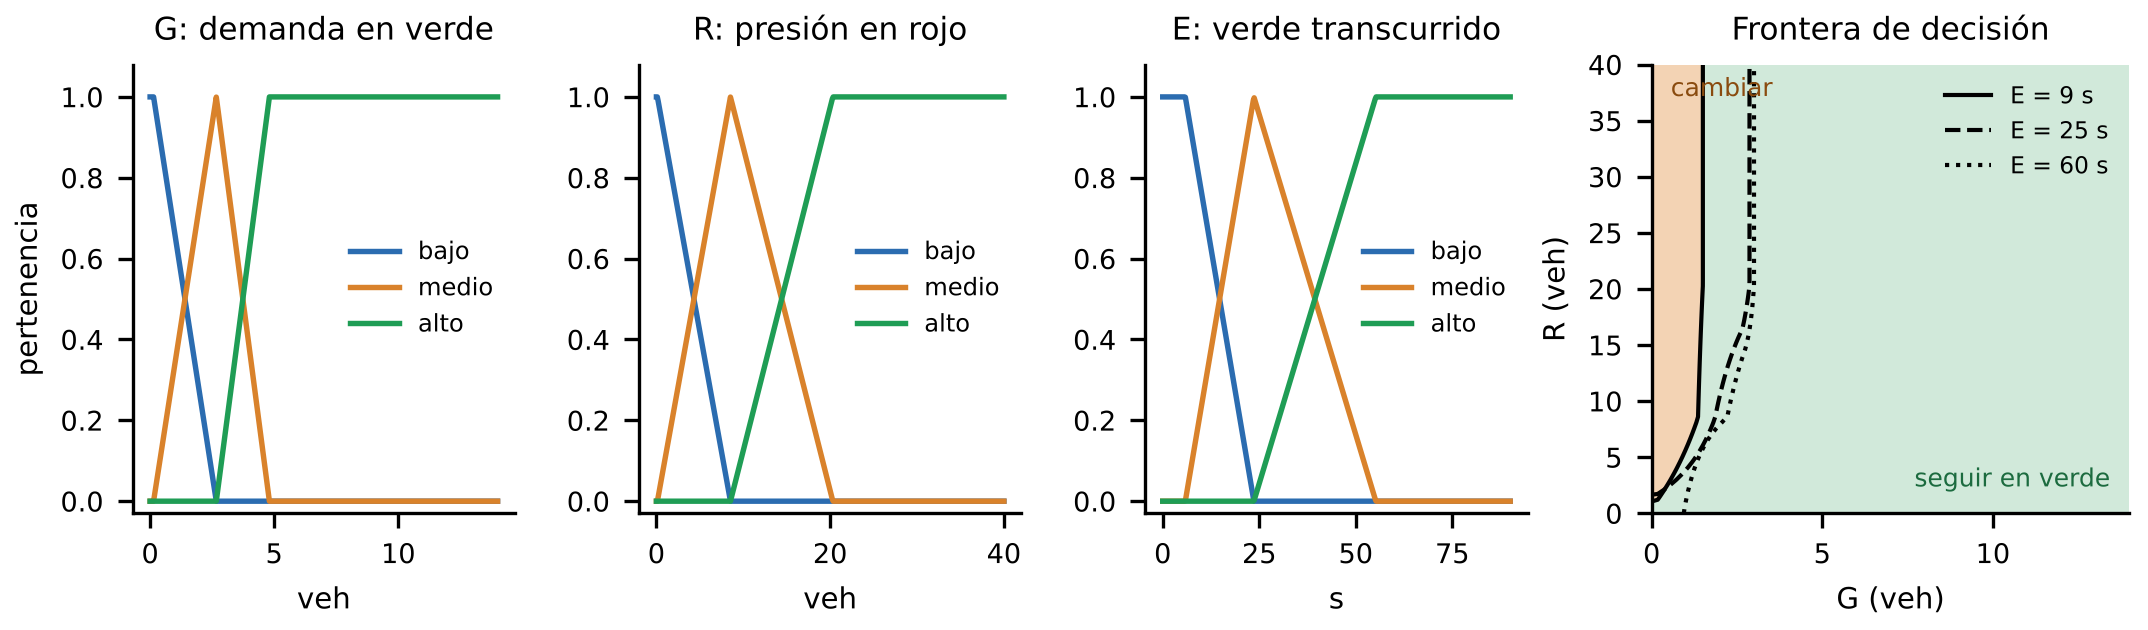
\includegraphics[width=\textwidth]{fig_opt_difuso.png}
\caption{Funciones de pertenencia aprendidas de \FLC{} para $G$, $R$ y $V$ y frontera de decisión $u=0$ en el plano $(G,R)$ para tres valores de $V$.}
\label{fig:difuso}
\end{figure*}

\begin{table}[t]
\centering
\caption{Base de reglas de FLC-O: consecuente num\'erico $c_{ijk}$ de cada regla (positivo: cambiar la fase; negativo: seguir en verde) seg\'un la demanda en verde $G$, la presi\'on en rojo $R$ y el verde transcurrido $V$. Nudos $(k_1,k_2,k_3)$: $G$ (0.1, 2.7, 4.8), $R$ (0.1, 8.5, 20.3), $V$ (5.9, 23.6, 55.2).}
\label{tab:reglasflc}
\scriptsize
\begin{tabular}{@{}llrrr@{}}
\toprule
$G$ & $R$ & $V$ bajo & $V$ medio & $V$ alto \\
\midrule
bajo & bajo & $-$0.15 & $-$0.47 & +1.60 \\
bajo & medio & +1.62 & +1.68 & +1.57 \\
bajo & alto & +1.34 & +1.49 & +1.37 \\
medio & bajo & $-$2.67 & $-$1.15 & $-$3.44 \\
medio & medio & $-$1.96 & $-$0.81 & $-$0.35 \\
medio & alto & $-$1.51 & +0.38 & +0.40 \\
alto & bajo & $-$1.27 & $-$1.73 & $-$2.27 \\
alto & medio & $-$1.68 & $-$1.34 & $-$0.08 \\
alto & alto & $-$0.62 & $-$3.74 & $-$2.20 \\
\bottomrule
\end{tabular}
\fuente{modelo entrenado flcs\_preview (resultados/opt/flcs\_preview.json).}
\end{table}


\subsection{Política neuronal}
\label{sec:neuronal}
Para saber qué tanto se pierde por exigir reglas legibles, se entrena también, con las mismas condiciones, una política opaca: un perceptrón de una capa oculta de 8 neuronas con tangente hiperbólica (121 parámetros) que recibe 12 características (colas, verde transcurrido, llegadas previstas en 3 y 10\,s, tasas de llegada de los últimos 5 y 20\,s, y si la cola del verde está vacía) y decide cada segundo. Es una referencia empírica de lo que logra un aprendizaje sin estructura con esa información; no es una cota, porque el entrenamiento puede quedar en un óptimo local, ni un controlador propuesto.

\subsection{Entrenamiento}
\label{sec:entrena}
Todos los parámetros se optimizan con CMA-ES \cite{Hansen2001,Hansen2016}: una estrategia evolutiva que adapta la covarianza de una distribución normal con la que sortea candidatos y que usa los mejores para actualizarla. El objetivo de un parámetro $\theta$ es
\begin{equation}
J(\theta)=\frac{1}{N}\sum_{i=1}^{N}\frac{d_m^{(i)}(\theta)}{d_m^{(i)}(\text{act})},
\label{eq:objetivo}
\end{equation}
la media sobre $N=64$ escenarios de entrenamiento (definición propia) del retardo \eqref{eq:dm} del controlador dividido por el del actuado afinado en el mismo escenario, de modo que $J<1$ significa mejor que el actuado y todos los niveles de demanda pesan igual. Los escenarios de entrenamiento son caudales sorteados al azar, con suma de 540 a 3300\,veh/h y semillas distintas de las de la prueba; no incluyen los 16 pares de la Tabla VIII. Cada evaluación simula 3600\,s por escenario. Con 4 procesos en paralelo, entrenar \FLC{} toma unos 15 minutos.

% =============================================================================
\section{Protocolo experimental}
\label{sec:protocolo}

\textbf{Controladores comparados} (Tabla~\ref{tab:controladores}). Además de los dos de Pappis y Mamdani y \FLC{}: el ciclo fijo de Webster; el actuado por detector de la réplica (verde mínimo 7\,s, máximo 57\,s, hueco 3\,s); un actuado afinado, cuyo hueco, verde mínimo y máximo se eligieron en los mismos escenarios de entrenamiento y dentro del mismo rango que los controladores entrenados (verde mínimo de 3 a 7\,s, máximo de 90\,s): resultó hueco de 1\,s, mínimo de 3\,s y máximo de 90\,s, para que el rival sea justo; la presión máxima \cite{Varaiya2013}, con parámetros afinados en el mismo rango; la cota óptima y la política neuronal.

\begin{table}[t]
\centering
\caption{Controladores comparados y la información que usan}
\label{tab:controladores}
\scriptsize
\setlength{\tabcolsep}{2.5pt}
\begin{tabular}{@{}lccc@{}}
\toprule
Controlador & Caudales & Vista adelante & Parámetros \\
\midrule
Ciclo fijo (Webster) & sí & no & 0 \\
Actuado, actuado afinado & no & no & 3 \\
Presión máxima & no & no & 3 \\
Pappis y Mamdani & no & 10 s & 0 \\
Pappis y Mamdani afinado & no & 10 s & 30 \\
Óptimo (programación dinámica) & sí & no & -- \\
FLC-O & no & 10 s (pesos aprendidos) & 42 \\
Política neuronal & no & 10 s & 121 \\
\bottomrule
\end{tabular}
\fuente{elaboración propia.}
\end{table}

\textbf{Conjuntos de prueba} (nunca usados para entrenar), todos de 7200\,s:
\begin{itemize}
\item \emph{Oficial}: los 16 pares de caudales de la Tabla VIII del original con 20 réplicas (semillas 0 a 19, números aleatorios comunes entre controladores).
\item \emph{No vistos}: 64 pares sorteados con otras semillas.
\item \emph{Variable}: 64 escenarios con demanda que cambia cada 600\,s con un factor de 0.4 a 1.6; se evalúa cómo se comportan controladores que no conocen los caudales.
\item \emph{Saturado}: 32 pares con suma de 3000 a 3300\,veh/h, cerca de la capacidad.
\end{itemize}

\textbf{Estadística.} En el conjunto oficial, para cada par de caudales se compara cada controlador con cada referencia con la prueba de rangos con signo de Wilcoxon sobre las 20 réplicas pareadas, con la corrección de Holm sobre los 16 pares, y se reportan la media, la desviación estándar muestral y el intervalo de confianza de 95\,\% (t de Student). La mejora de un par es la reducción relativa del retardo medio. Todo el código y los resultados están en el repositorio (Sección~\ref{sec:disp}).

% =============================================================================
\section{Resultados}
\label{sec:resultados}

\subsection{Conjunto oficial: Tabla VIII}
\label{sec:res-oficial}
La Tabla~\ref{tab:oficial} y la Fig.~\ref{fig:retardo} muestran el retardo en los 16 pares. El retardo medio es de \DelayOfFijo{}\,s/veh con el ciclo fijo, \DelayOfPap{} con Pappis y Mamdani, \DelayOfActAf{} con el actuado afinado y \DelayOfFlc{} con \FLC{}, es decir, una reducción de \RedFlc\,\% respecto de Pappis y Mamdani. Por par de caudales, la mejora media es de \ParMediaPap\,\% (de \ParMinPap\,\% a \ParMaxPap\,\%) y es significativa en \ParMejorPap{} de 16 pares, sin ningún par significativamente peor (Tabla~\ref{tab:comparaciones}). Frente al actuado afinado, que es un rival más fuerte que el original, la mejora media es de \ParMediaActAf\,\%, significativa en \ParMejorActAf{} pares y en contra en \ParPeorActAf{}. La cota óptima, que conoce los caudales pero no ve el futuro, da \DelayOfMdp{}\,s/veh: \FLC{} la iguala o la supera en promedio porque sí ve las llegadas de los próximos segundos, y no porque la cota sea defectuosa.

\begin{table}[t]
\centering
\caption{Retardo medio por veh\'iculo (s) en los 16 pares de caudales de la Tabla VIII del art\'iculo original, con 20 r\'eplicas de 7200 s y n\'umeros aleatorios comunes. Se cuenta la espera de todos los veh\'iculos hasta el horizonte. $\Delta$: mejora de FLC-O frente a Pappis y Mamdani (\%); $^{*}$: significativa (Wilcoxon pareado, Holm, 0.05). En negrita, el menor de las cuatro primeras columnas.}
\label{tab:oficial}
\scriptsize
\setlength{\tabcolsep}{2.6pt}
\begin{tabular}{@{}lrrrrrr@{}}
\toprule
N-S / E-W (veh/h) & Webster & Actuado af. & Pappis & FLC-O & $\Delta$ (\%) & \'Optimo$^{\dagger}$ \\
\midrule
360 / 360 & 7.30 & 5.81 & 5.58 & \textbf{4.47} & +19.9$^{*}$ & 5.01 \\
360 / 720 & 7.49 & 6.46 & 5.97 & \textbf{4.93} & +17.4$^{*}$ & 5.61 \\
360 / 1080 & 7.77 & 7.08 & 6.25 & \textbf{5.50} & +12.1$^{*}$ & 5.86 \\
360 / 1440 & 8.26 & 7.74 & 6.70 & \textbf{6.19} & +7.6$^{*}$ & 6.26 \\
360 / 1800 & 9.22 & 8.45 & 7.40 & \textbf{6.98} & +5.7$^{*}$ & 6.90 \\
360 / 2160 & 11.34 & 9.36 & 8.71 & \textbf{8.12} & +6.7$^{*}$ & 7.99 \\
360 / 2520 & 16.31 & 10.83 & 12.02 & \textbf{10.72} & +10.9$^{*}$ & 9.95 \\
720 / 720 & 9.36 & 7.45 & 6.57 & \textbf{6.16} & +6.3$^{*}$ & 7.04 \\
720 / 1080 & 10.65 & 8.33 & 7.54 & \textbf{7.19} & +4.7$^{*}$ & 7.88 \\
720 / 1440 & 12.53 & 9.39 & 9.34 & \textbf{8.53} & +8.7$^{*}$ & 9.01 \\
720 / 1800 & 15.38 & 10.92 & 12.21 & \textbf{10.36} & +15.1$^{*}$ & 10.70 \\
720 / 2160 & 21.27 & 13.75 & 17.69 & \textbf{13.72} & +22.4$^{*}$ & 13.63 \\
1080 / 1080 & 13.56 & 9.66 & 9.78 & \textbf{8.99} & +8.1$^{*}$ & 9.58 \\
1080 / 1440 & 17.81 & 11.82 & 13.82 & \textbf{11.45} & +17.2$^{*}$ & 11.79 \\
1080 / 1800 & 25.68 & \textbf{15.86} & 22.41 & 16.09 & +28.2$^{*}$ & 15.89 \\
1440 / 1440 & 26.98 & \textbf{16.45} & 23.24 & 16.79 & +27.8$^{*}$ & 16.44 \\
\midrule
Media & 13.81 & 9.96 & 10.95 & 9.14 & +13.7 & 9.35 \\
\bottomrule
\end{tabular}
\fuente{simulaci\'on del autor (resultados/opt/evaluacion\_final.json); $^{\dagger}$ cota por programaci\'on din\'amica que conoce los caudales y no ve llegadas futuras (Sec.~\ref{sec:pd}).}
\end{table}

\begin{table}[t]
\centering
\caption{FLC-O frente a cada referencia en la Tabla VIII: mejora media del retardo por par de caudales (\%), intervalo de las 16 mejoras y n\'umero de pares (de 16) en que es significativamente mejor o peor (Wilcoxon pareado sobre 20 r\'eplicas, correcci\'on de Holm, 0.05).}
\label{tab:comparaciones}
\scriptsize
\begin{tabular}{@{}lrrrr@{}}
\toprule
Referencia & Mejora media & Intervalo & Mejor & Peor \\
\midrule
Pappis y Mamdani & +13.7 & +4.7 a +28.2 & 16 & 0 \\
Ciclo fijo (Webster) & +32.8 & +24.3 a +38.7 & 16 & 0 \\
Actuado (hueco 3 s) & +18.5 & +7.0 a +31.8 & 16 & 0 \\
Actuado afinado & +10.8 & $-$2.1 a +23.6 & 12 & 2 \\
\bottomrule
\end{tabular}
\fuente{simulaci\'on del autor; Wilcoxon exacto o con aproximaci\'on normal seg\'un empates (estadistica.py).}
\end{table}


\begin{figure*}[!t]
\centering
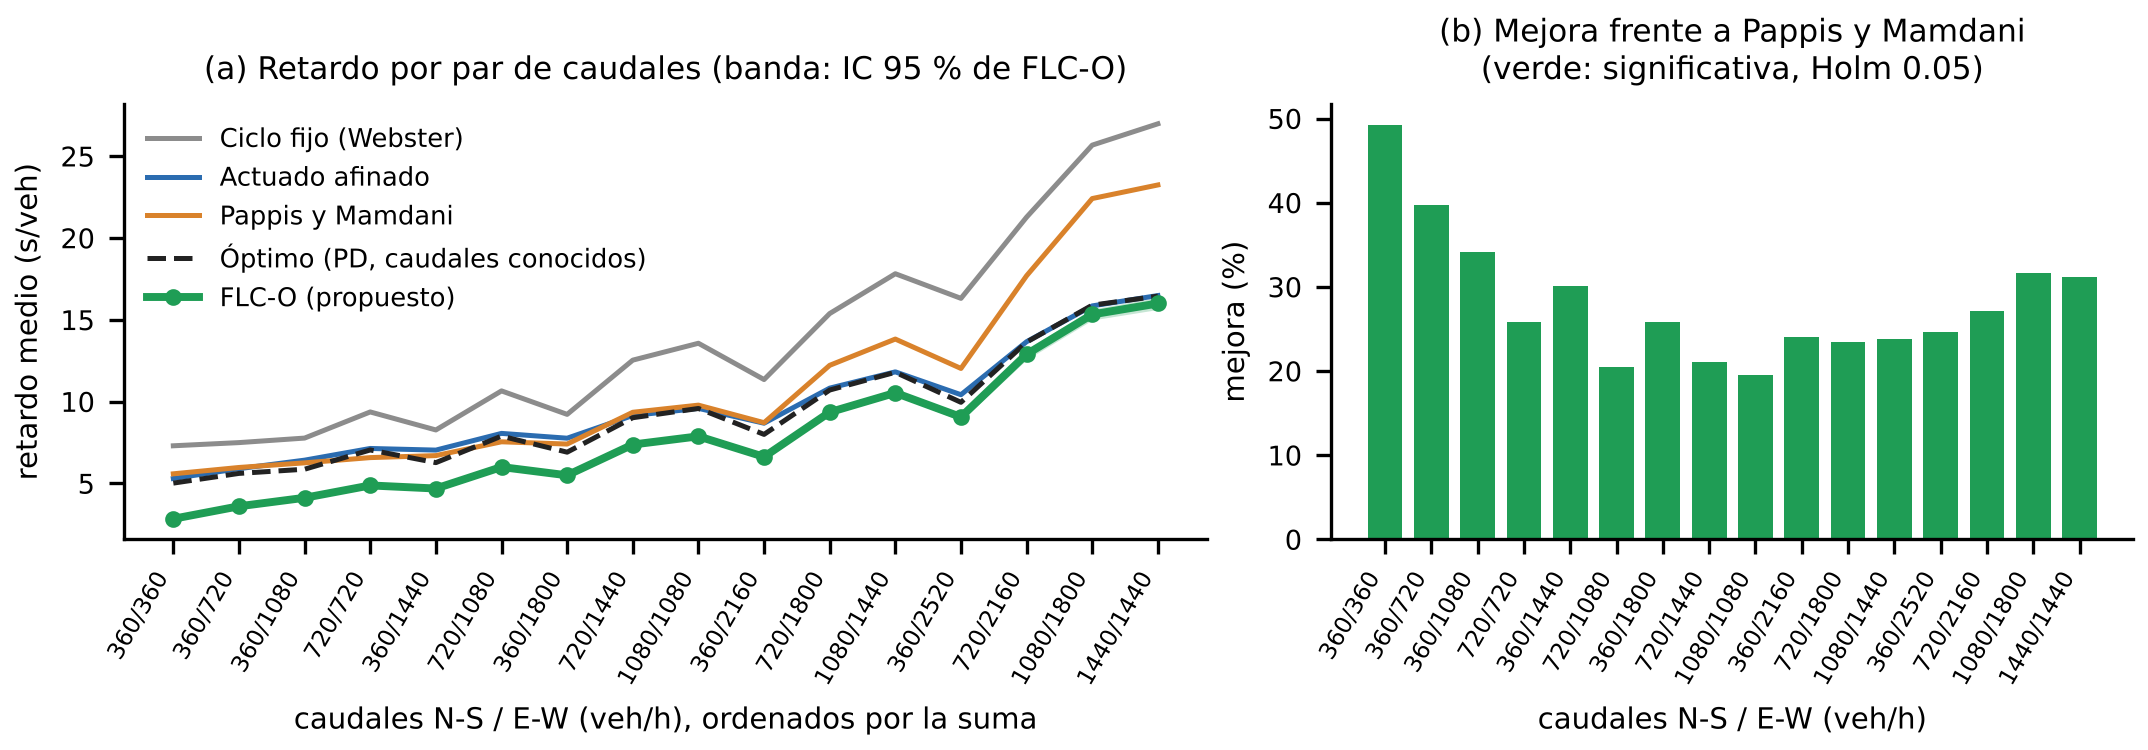
\includegraphics[width=\textwidth]{fig_opt_retardo.png}
\caption{(a) Retardo medio por par de caudales de la Tabla VIII (7200\,s, 20 réplicas); la banda es el intervalo de confianza de 95\,\% de \FLC{}. (b) Mejora de \FLC{} frente a Pappis y Mamdani en cada par; en verde, las significativas con la corrección de Holm.}
\label{fig:retardo}
\end{figure*}

\subsection{Caudales no vistos, demanda variable y saturación}
\label{sec:res-otros}
La Tabla~\ref{tab:conjuntos} resume los otros conjuntos. Con 64 pares de caudales no vistos, \FLC{} reduce el retardo en \RedPapNv\,\% frente a Pappis y Mamdani y en \RedActAfNv\,\% frente al actuado afinado, de modo que la mejora no depende de los 16 pares de la Tabla VIII. Con demanda variable, que es donde un controlador que adapta su decisión a lo que ve debería ganar más, las reducciones son de \RedPapVa\,\% y \RedActAfVa\,\%, y superan a las del caso estacionario. Cerca de la saturación el resultado es distinto: el retardo medio de \FLC{} es de \DelaySaFlc{}\,s/veh, el de Pappis y Mamdani de \DelaySaPap{} y el del actuado afinado de \DelaySaActAf{}. Se discute en la Sección~\ref{sec:discusion}.

\begin{table}[t]
\centering
\caption{Retardo medio (s/veh) en los conjuntos de prueba. Oficial: Tabla VIII, 16 pares $\times$ 20 r\'eplicas. No vistos: 64 pares sorteados con otras semillas. Variable: demanda por tramos de 600 s con factor de 0.4 a 1.6. Saturado: suma de caudales de 3000 a 3300 veh/h. Todos con 7200 s.}
\label{tab:conjuntos}
\scriptsize
\begin{tabular}{@{}lrrrr@{}}
\toprule
Controlador & Oficial & No vistos & Variable & Saturado \\
\midrule
Ciclo fijo (Webster) & 13.8 & 12.3 & 12.3 & 40.7 \\
Actuado (hueco 3 s) & 10.9 & 10.2 & 9.2 & 54.1 \\
Actuado afinado & 10.0 & 9.2 & 8.4 & 23.2 \\
Presión máxima & 31.2 & 23.5 & 16.9 & 351.0 \\
Pappis y Mamdani & 11.0 & 10.0 & 8.7 & 105.9 \\
Pappis y Mamdani afinado & 9.7 & 9.1 & 8.0 & 62.1 \\
FLC-O (propuesto) & 9.1 & 8.3 & 7.3 & 48.7 \\
Óptimo (PD, caudales conocidos) & 9.3 & 8.5 & 7.9 & 23.1 \\
Política neuronal (cota) & 8.7 & 7.9 & 6.9 & 54.3 \\
\bottomrule
\end{tabular}
\fuente{simulaci\'on del autor (resultados/opt/evaluacion\_final.json). El \'optimo no se calcula en el conjunto saturado (la cola truncada de la programaci\'on din\'amica no es fiable all\'i).}
\end{table}


\subsection{Qué produce la mejora}
\label{sec:res-abl}
La Tabla~\ref{tab:ablacion} compara variantes entrenadas con las mismas condiciones, de modo que cada fila cambia un solo factor.
(i) Afinar solo las 25 reglas de Pappis y Mamdani da \DelayOfPapAf{}\,s/veh en el conjunto oficial: parte de la mejora viene del ajuste, pero no toda.
(ii) El verde mínimo es el factor que más pesa: con $g_{\min}$ de 7, 5, 4 y 3\,s, \FLC{} da \DelayOfGSiete{}, \DelayOfGCinco{}, \DelayOfGCuatro{} y \DelayOfSemDos{}\,s/veh. Con 5\,s se conserva casi toda la mejora (\RedPapGCinco\,\% frente a Pappis y Mamdani, contra \RedFlc\,\% con 3\,s), lo que importa si la norma local exige un verde mínimo mayor.
(iii) Aprender los pesos de la vista adelante ayuda: con horizontes fijos, el mismo difuso de 27 reglas y 36 parámetros da \DelayOfFijos{}\,s/veh frente a \DelayOfSemDos{} de \FLC{}.
(iv) Cuatro veces más reglas (81, con el tiempo desde la última llegada como cuarta variable) da \DelayOfReglas{}\,s/veh, sin mejora: la base de 27 reglas basta.
(v) La política neuronal de 121 parámetros, entrenada igual, da \DelayOfMlp{}\,s/veh, no mejor que \FLC{}: exigir reglas legibles no cuesta desempeño aquí, y la red no es una cota.
(vi) Sin vista adelante, \FLC{} causal da \DelayOfFlcC{}\,s/veh, la política lineal con hueco \DelayOfLinC{} y la neuronal \DelayOfMlpC{}, frente a \DelayOfActAf{} del actuado afinado: la mejor, la neuronal, lo mejora solo en \RedActMlpC\,\% y \FLC{} causal queda en \RedActFlcC\,\%, contra \RedActAfOf\,\% de \FLC{} con vista adelante. La mayor parte de la mejora depende de ver el futuro cercano.

\begin{table}[t]
\centering
\caption{Variantes de FLC-O y controladores aprendidos. Retardo medio (s/veh) en la Tabla VIII, en caudales no vistos y con demanda variable. $g_{\min}$: verde m\'inimo.}
\label{tab:ablacion}
\scriptsize
\setlength{\tabcolsep}{2.4pt}
\begin{tabular}{@{}lrlrrr@{}}
\toprule
Variante & Par. & Informaci\'on & Oficial & No vistos & Variable \\
\midrule
Pappis y Mamdani afinado & 30 & vista adelante & 9.69 & 9.1 & 8.0 \\
Difuso 27 reglas ($g_{\min}=7$) & 36 & vista adelante & 9.14 & 8.3 & 7.3 \\
Difuso 81 reglas con hueco & 93 & vista adelante & 9.16 & 8.5 & 7.3 \\
Difuso 27 reglas, causal & 36 & solo pasado & 10.53 & 9.8 & 9.0 \\
Política neuronal & 121 & vista adelante & 8.68 & 7.9 & 6.9 \\
Política neuronal, causal & 121 & solo pasado & 10.17 & 9.6 & 8.8 \\
\bottomrule
\end{tabular}
\fuente{simulaci\'on del autor; par.: n\'umero de par\'ametros entrenados.}
\end{table}


\begin{figure*}[!t]
\centering
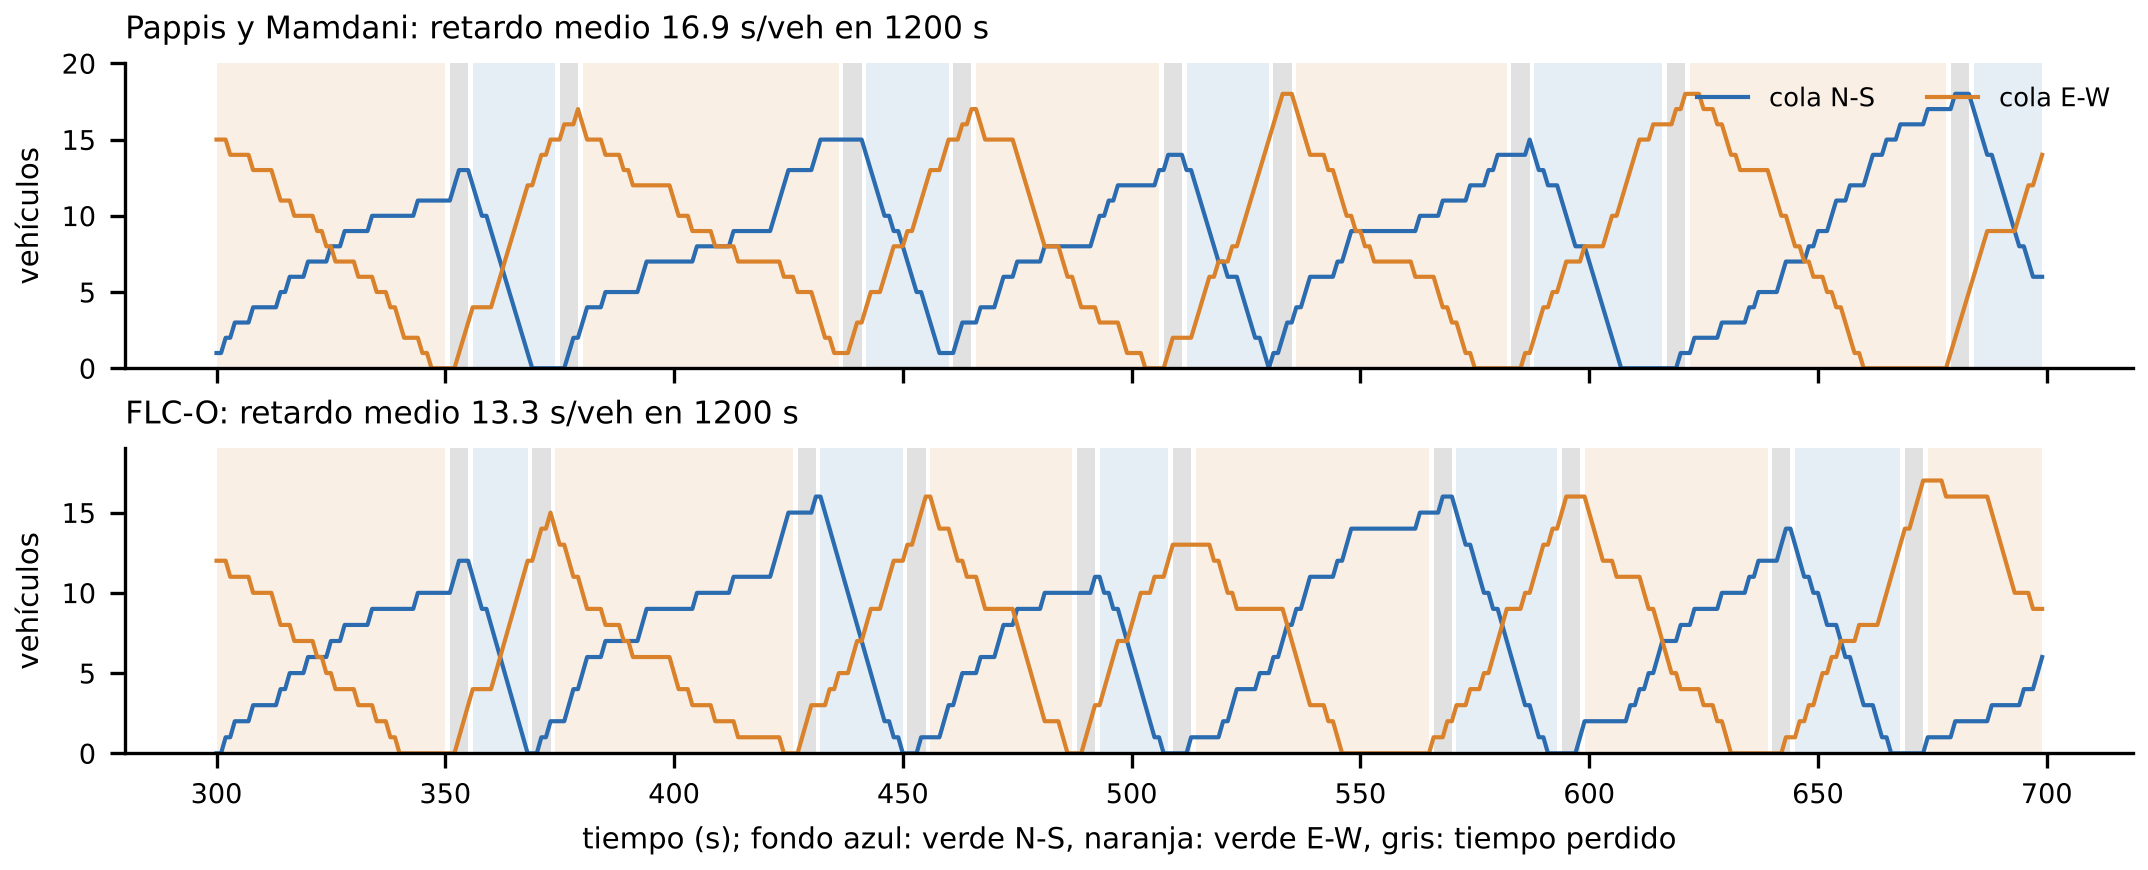
\includegraphics[width=\textwidth]{fig_opt_traza.png}
\caption{Colas y fases durante 400\,s en un escenario de 720/2160\,veh/h con las mismas llegadas: Pappis y Mamdani (arriba) y \FLC{} (abajo). El fondo indica el brazo con verde y, en gris, el tiempo perdido.}
\label{fig:traza}
\end{figure*}

% =============================================================================
\section{Discusión}
\label{sec:discusion}

\textbf{Qué se logró.} Dentro del modelo del original, un controlador difuso de 27 reglas y 42 parámetros entrenado con caudales sorteados reduce el retardo en \RedFlc\,\% frente al de 1977 en la Tabla VIII, y en \RedActAfOf\,\% frente a un actuado afinado con el mismo rango de parámetros, que es una referencia más exigente que la del original. La mejora se mantiene con caudales no vistos (\RedPapNv\,\% y \RedActAfNv\,\%) y con demanda variable (\RedPapVa\,\% y \RedActAfVa\,\%). Según la ablación, las razones son tres: decide cada segundo y no cada 10\,s, admite un verde mínimo menor, y mide la demanda y la presión con pesos de la vista adelante aprendidos y no con las tablas fijas de 1977. La variación entre semillas de entrenamiento es pequeña (Tabla~S3 del suplemento).

\textbf{Qué no se logró.} (i) La mejora depende de la vista adelante de 10\,s. Es un supuesto del original, que equivale a detectores aguas arriba sin error de medición, y es optimista en la práctica. Sin ella, el mejor controlador aprendido mejora al actuado afinado solo en \RedActMlpC\,\% y el difuso causal no lo mejora. (ii) Cerca de la saturación el desempeño de \FLC{} es de \DelaySaFlc{}\,s/veh frente a \DelaySaActAf{} del actuado afinado y \DelaySaPap{} de Pappis y Mamdani; el rango de entrenamiento y el verde máximo limitan la extrapolación. (iii) El verde mínimo de 3\,s elegido por validación puede no ser admisible en una intersección real, por seguridad y por la norma local; con 5\,s la ganancia es de \RedPapGCinco\,\% frente a Pappis y Mamdani. (iv) Todo es simulación con llegadas de Bernoulli, un solo cruce y un flujo de saturación fijo; no hay datos de campo, ni giros, ni peatones, ni redes. (v) El retardo corregido no es el que imprimía el original, por lo que las cifras no son comparables con las de su Tabla VIII.

\textbf{Amenazas a la validez.} Los parámetros se entrenaron con el mismo simulador con el que se evalúan, aunque con caudales y semillas distintos; un simulador distinto, o datos reales, podrían cambiar las conclusiones. El actuado afinado y la presión máxima se afinaron con los mismos escenarios, el mismo rango de verde mínimo y el mismo verde máximo que \FLC{}, pero no hay garantía de que sean los mejores de su clase. El verde mínimo y la semilla de \FLC{} se eligieron con los escenarios de validación, no con los de prueba; se reportan las tres semillas y los cuatro verdes mínimos. La política neuronal no es una cota: otra arquitectura o más entrenamiento podrían superarla.

% =============================================================================
\section{Conclusiones}
\label{sec:conclusiones}

Se pudo mejorar el controlador difuso de Pappis y Mamdani. Con un procedimiento reproducible (simulador vectorizado exacto, objetivo que cuenta toda la espera, entrenamiento con CMA-ES en caudales sorteados y prueba separada), un controlador difuso de 27 reglas y 42 parámetros reduce el retardo medio en \RedFlc\,\% en la Tabla VIII del original, es significativamente mejor en \ParMejorPap{} de 16 pares de caudales y mejora en \RedActAfOf\,\% a un actuado afinado con el mismo rango de parámetros. La mejora se mantiene con caudales no vistos y con demanda variable, depende de la vista adelante que el original ya supone (sin ella, el mejor controlador aprendido mejora al actuado afinado solo en \RedActMlpC\,\%) y no se mantiene cerca de la saturación. Como trabajo futuro quedan la robustez ante errores de medición de la vista adelante, el entrenamiento con un rango de caudales que cubra la saturación y la validación con datos de campo.

% =============================================================================
\section*{Disponibilidad del código}
\label{sec:disp}
El código, las pruebas, los resultados y el simulador están en la rama \texttt{optimizacion} del repositorio público \url{https://github.com/INVESTVALQUISP/PROYECTO_INVESTIGACION/tree/optimizacion}; la rama \texttt{main} conserva la réplica. Las pruebas se ejecutan con \texttt{python codigo/ejecutar\_pruebas.py}; el entrenamiento, con \texttt{codigo/opt\_entrenar\_modelo.py}; la evaluación final, con \texttt{codigo/opt\_evaluacion\_final.py}; y las tablas y figuras de este artículo se regeneran con \texttt{codigo/gen\_tablas\_opt.py} y \texttt{codigo/gen\_fig\_opt.py}. Los resultados están en \texttt{resultados/opt/}. Python 3.13, NumPy 2.5 y semillas de PCG64 fijas.

\bibliographystyle{IEEEtran}
\bibliography{referencias}

\end{document}
